\documentclass[11pt,a4paper]{article}

\usepackage[margin=1in, paperwidth=8.3in, paperheight=11.7in]{geometry}
\usepackage{amsfonts}
\usepackage{amsmath}
\usepackage{amssymb}
\usepackage{array}
\usepackage{enumerate}
\usepackage{enumitem}
\usepackage{fancyhdr}
\usepackage{graphicx}
\usepackage{tikz}
\usepackage{changepage} 
\usepackage{longtable} 

\begin{document}

\pagestyle{fancy}
\setlength\parindent{0pt}
\allowdisplaybreaks

\renewcommand{\headrulewidth}{0pt}

%New column type
\newcolumntype{L}[1]{>{\arraybackslash}m{#1cm}}

% Cover page title
\title{Image Processing and Computer Vision - Notes}
\author{Dom Hutchinson}
\date{\today}
\maketitle

% Header
\fancyhead[L]{Dom Hutchinson}
\fancyhead[C]{Image Processing and Computer Vision - Notes}
\fancyhead[R]{\today}

% Counters
\newcounter{definition}[section]
\newcounter{example}[section]
\newcounter{notation}[section]
\newcounter{proposition}[section]
\newcounter{remark}[section]
\newcounter{theorem}[section]
\newcounter{proof}[section]

% commands
\newcommand{\dotprod}[0]{\boldsymbol{\cdot}}
\newcommand{\cosech}[0]{\mathrm{cosech}\ }
\newcommand{\cosec}[0]{\mathrm{cosec}\ }
\newcommand{\sech}[0]{\mathrm{sech}\ }
\newcommand{\blocks}[0]{\mathbb{B}}
\newcommand{\nats}[0]{\mathbb{N}}
\newcommand{\reals}[0]{\mathbb{R}}
\newcommand{\integers}[0]{\mathbb{Z}}
\newcommand{\nb}[0]{\textit{N.B.} }
\newcommand{\ie}[0]{\textit{i.e.} }
\newcommand{\eg}[0]{\textit{e.g.} }

\newcommand{\definition}[1]{\stepcounter{definition} \textbf{Definition \arabic{section}.\arabic{definition}\ - }\textit{#1}\\}
\newcommand{\example}[1]{\stepcounter{example} \textbf{Example \arabic{section}.\arabic{example}\ - }\textit{#1}\\}
\newcommand{\notation}[1]{\stepcounter{notation} \textbf{Notation \arabic{section}.\arabic{notation}\ - }\textit{#1}\\}
\newcommand{\proposition}[1]{\stepcounter{proposition} \textbf{Proposition \arabic{section}.\arabic{proposition}\ - }\textit{#1}\\}
\newcommand{\remark}[1]{\stepcounter{remark} \textbf{Remark \arabic{section}.\arabic{remark}\ - }\textit{#1}\\}
\newcommand{\theorem}[1]{\stepcounter{theorem} \textbf{Theorem \arabic{section}.\arabic{theorem}\ - }\textit{#1}\\}
\newcommand{\proof}[1]{\stepcounter{proof} \textbf{Proof \arabic{section}.\arabic{proof}\ - }\textit{#1}\\}
\newcommand{\definitionn}[1]{\stepcounter{definition} \textbf{Definition \arabic{section}.\arabic{definition}\ - }\textit{#1}}
\newcommand{\examplee}[1]{\stepcounter{example} \textbf{Example \arabic{section}.\arabic{example}\ - }\textit{#1}}
\newcommand{\notationn}[1]{\stepcounter{notation} \textbf{Notation \arabic{section}.\arabic{notation}\ - }\textit{#1}}
\newcommand{\propositionn}[1]{\stepcounter{proposition} \textbf{Proposition \arabic{section}.\arabic{proposition}\ - }\textit{#1}}
\newcommand{\remarkk}[1]{\stepcounter{remark} \textbf{Remark \arabic{section}.\arabic{remark}\ - }\textit{#1}}
\newcommand{\theoremm}[1]{\stepcounter{theorem} \textbf{Theorem \arabic{section}.\arabic{theorem}\ - }\textit{#1}}
\newcommand{\prooff}[1]{\stepcounter{proof} \textbf{Proof \arabic{section}.\arabic{proof}\ - }\textit{#1}}


\tableofcontents

% Start of content
\newpage

\section{Image Acquistion}

\proposition{Common Challenges with Image Acquistion}
Below are some common challeges that are faced/produced by image acquistion\\
\begin{tabular}{|l|L{12}|}
\hline
Viewpoint Variation&Several images may be taken of the same object but will vary the angle\\
Illumination&Images may be taken in low/high light\\
Occlusion&Object may be partly obscured\\
Scale&Objects may look vary different when placed next to other objects due to their relative scale\\
Deformation&Objects may have slight variations on the perfect form\\
Background Clutter&Lots happening behind an object may work to obscure it\\
Object Intra-Class Variation&Some objects in the same class can vary a lot in shape (\eg chairs)\\
Local Ambiguity&Certain regions of an image can be missinturpred without the rest of the scene being accounted for\\
World Behind the Image&Depth may need to be accounted for to make sense of an image.\\
\hline
\end{tabular}\\

\definition{Dirac Delta-Function, $\delta$}
The \textit{Dirac Delta-Function} is used to map continuous distributions to discrete distributions by sampling at particular intervals. Intuitively
$$\delta(t)=\begin{cases}1&, t=0\\0&, t\neq0\end{cases}\implies\delta(t-\alpha)=\begin{cases}1&, t=\alpha\\0&, t\neq\alpha\end{cases}$$

\definition{Sifting Property}
We can apply the \textit{Dirac Delta-Function} to a function to sample a particular value
$$\int_{-\infty}^\infty f(t)\delta(t)dt=f(0)\implies\int_{-\infty}^\infty f(t)\delta(t-\alpha)dt=f(\alpha)$$
This can be applied to 2D objects (such as images) as
$$\int_{-\infty}^\infty f(a,b)\delta(a-x,b-y)dadb=f(x,y)$$

\definition{Point Spread-Function}
A \textit{Point Spread-Function} is applied after sampling an image. It takes the value of a pixel \& transforms pixels around it using this value in some way.\\
\eg\raisebox{-0.5\height}{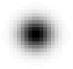
\includegraphics[scale=1]{img/psf.png}} (Should be a white dot on black background but ink).

\section{Image Representation}

\definition{Colour Space}
\textit{Colour Space} are different techniques for representing colours. These are generally made up of 3D vectors.\\
\begin{tabular}{|l|L{13}|}
\hline
Colour Space&Vector Description\\
\hline
RGB&(Red $\in[0,255]$,Green $\in[0,255]$,Blue $\in[0,255]$)\\
HSI&(Hue $\in[0,360)$,Saturation $\in[0,1]$,Intensity $\in[0,1]$)\newline Hue gives the colour in degrees\\
YUV&(Brightness $\in[0,255]$,Blue Projection $\in[0,255]$,Red Projection $\in[0,255]$)\\
La*b*&(Luminance $\in[0,100]$, Red/Green $\in\{-a,+b\}$, Blue/Yellow $\in\{+b,-b\}$\\
\hline
\end{tabular}\\

\remark{Representing Video}
To represent video each fixel is given a third parameter, $time$ so we now have
$$f(x,y,t)\mapsto(R,G,B)$$
or any other \textit{Colour Space}.\\

\definition{Quantisation}
\textit{Quantisation} is representing a continuous single channel function with discrete single channel function that groups the continuous values into a set number of levels.\\

\example{Quantisation}
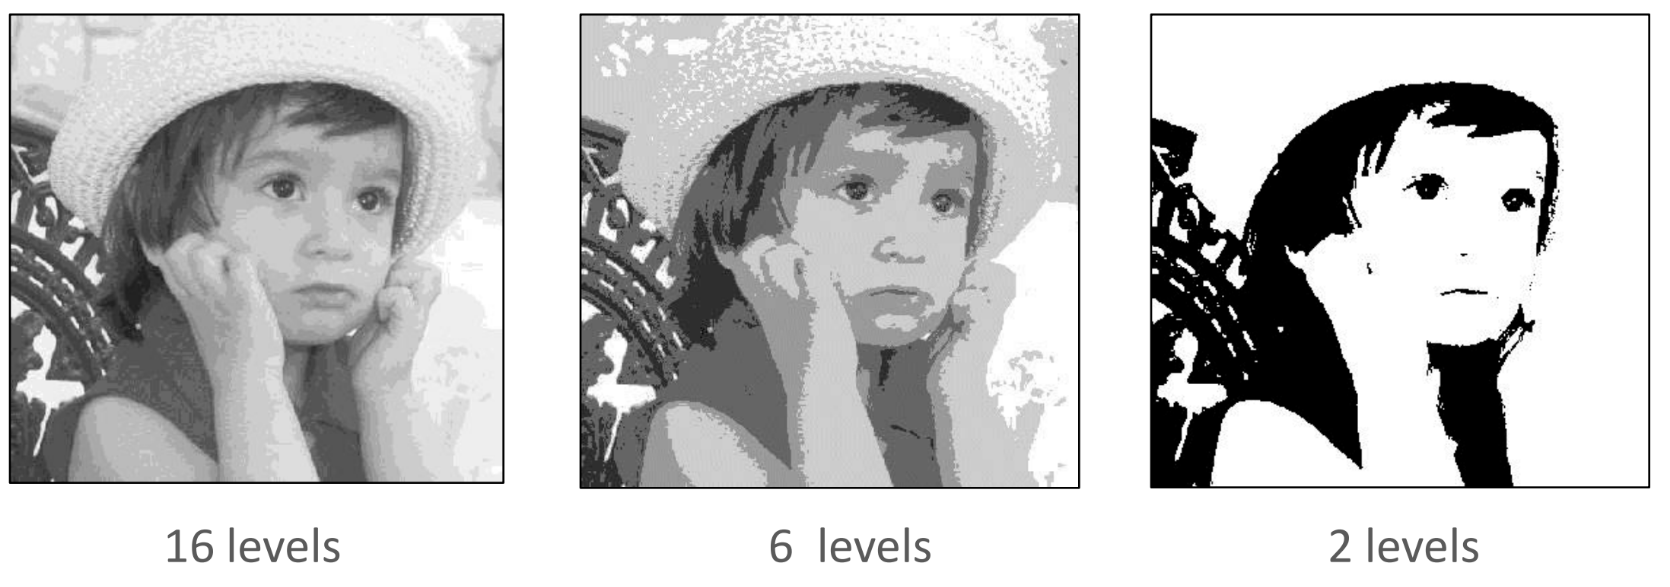
\includegraphics[scale=.3]{img/quantisation.png}

\definition{Aliasing}
\textit{Aliasing} is the result of sparse sampling since single pixels represent to large an area to get any detail out of it.\\

\example{Aliasing}
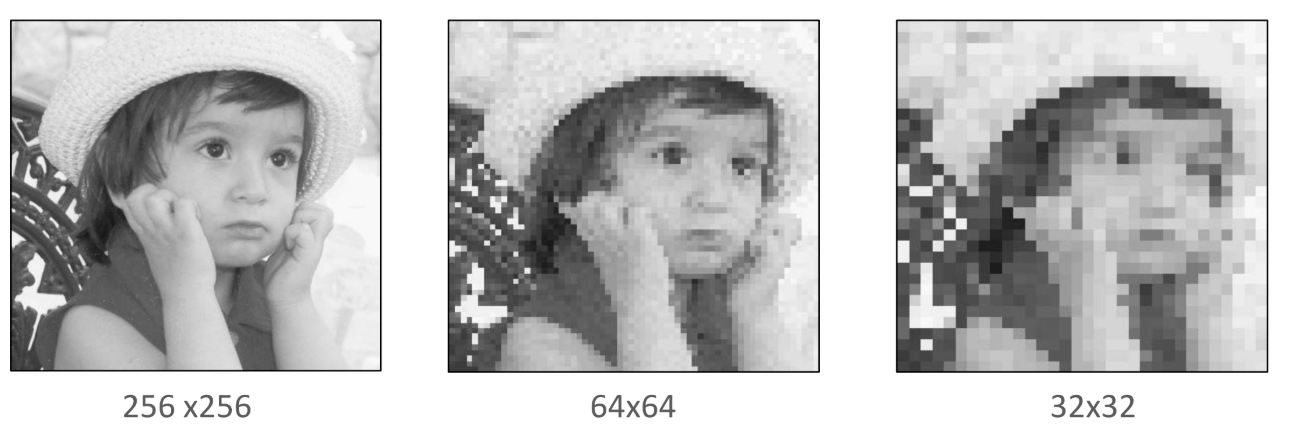
\includegraphics[scale=.4]{img/aliasing.png}

\definition{Anti-Aliasing}
\textit{Anti-Aliasing} is the process for avoiding \textit{Aliasing}. This can be achieved by using a sampling rate which is a critical limit defined by the \textit{Shannon-Nyquist Theorem}.\\

\theorem{Shannon-Nyquist Theorem}
An analogue signal with maximum frequency $x\text{Hz}$ may be completley reconstructed if regular samples are taken with frequency $2x\text{Hz}$.\\

\definition{Convolution}
\textit{Convolution} is an operation which takes two functions \& produces a third which describes how the shape of one of the two functions is changed by the other.\\
For functions $f\ \&\ g$
$$(f*g)(x):=\int_{-\infty}^\infty f(x-t)h(x)\partial t$$
\nb $*$ is the symbol for convolution.\\

\remark{Convolution in Image Representation}
Suppose you have a system, represented by kernel $g(x)$, \& an input signal, represented by $f(x)$. THen $f*g(x)$ describes the effect of the system on the input signal. The resulting image is called the \textit{Response of $f$ to the kernel $h$}.\\
%TODO what is a kernel

\proposition{2D Discrete Convolution}
Since images are represnted by discrete 2D functions $f:\nats\times\nats\to(\nats\times\nats\times\nats)$ it is pertinent to understand \textit{2D Discrete Convolution}.\\
$$h(x,y)=\sum_{i\in I}\sum_{j\in J}f(x-i,y-j)g(i,j)$$
Often the kernel, $g(x,y)$, has negative indices so the pixel being acted upto is equivalent to the middle pixel in the matrix representation of $g(x,y)$.\\
\nb A convolution whose kernel is symmetric on 180 degree rotation is called a \textit{Correlation}.\\

\example{2D Discrete Convolution}
Below is a representation of a grayscale image, $f(x,y)$, on the left \& a kernel $g(x,y)$ on the right.
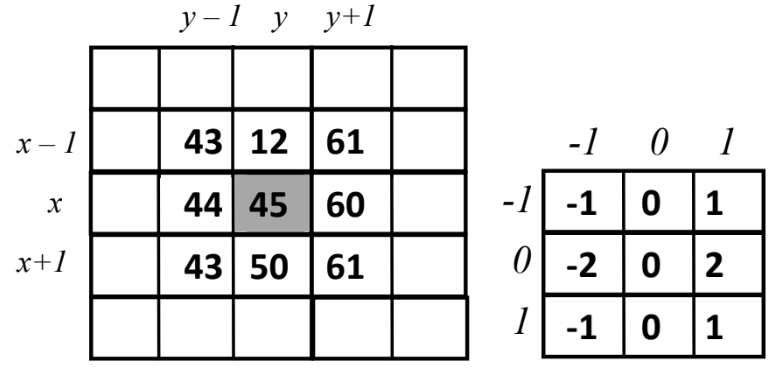
\includegraphics[scale=.3]{img/2dconvolution.png}\\
$(f*g)(x,y)=f(x+1,y+1)g(-1,-1)+f(x+1,y)g(0-1,0)+\dots+f(x-1,y-1)g(1,1)=-68$.\\

\example{Kernels}
Kernels an be defined with specific outcomes in mind.\\
\begin{longtable}{|l|l|}
\hline
\textbf{Operation}&\textbf{Matrix}\\
\hline
Identity&$\begin{pmatrix}
0&0&0\\
0&1&0\\
0&0&0
\end{pmatrix}$\\
\hline
Edge Detection&$\begin{pmatrix}
1&0&-1\\
0&0&0\\
-1&0&1
\end{pmatrix}$\\
&$\begin{pmatrix}
0&1&0\\
1&-4&1\\
0&1&1
\end{pmatrix}$\\
&$\begin{pmatrix}
-1&-1&-1\\
-1&8&-1\\
-1&-1&-1
\end{pmatrix}$\\
\hline
Sharpen&$\begin{pmatrix}
0&-1&0\\
-1&5&-1\\
0&-1&0
\end{pmatrix}$\\
\hline
Box Blur&$\dfrac{1}{9}\begin{pmatrix}
1&1&1\\
1&1&1\\
1&1&1
\end{pmatrix}$
\\
\hline
Gaussian Blur $3\times3$&$\dfrac{1}{16}\begin{pmatrix}
1&2&1\\
2&4&2\\
1&2&1
\end{pmatrix}$\\
\hline
Gaussian Blur $5\times5$&$\dfrac{1}{256}\begin{pmatrix}
1&4&6&4&1\\
4&16&24&16&4\\
6&24&36&24&6\\
4&16&24&16&4\\
1&4&5&4&1
\end{pmatrix}$\\
\hline
Unsharp Masking $5\times5$&$\dfrac{-1}{256}\begin{pmatrix}
1&4&6&4&1\\
4&16&24&16&4\\
6&24&-476&24&6\\
4&16&24&16&4\\
1&4&6&4&1
\end{pmatrix}$\\
\hline
\end{longtable}

\section{Frequency Domains \& Image Transforms}

\definition{Image Transform}
An \textit{Image Transform} is deriving a new representation of the input data by encoding the image using another parameter space (\eg Fourier, DCT, Wavelet, etc.).\\

\remark{Purpose of Image Transforms}
\textit{Image Transforms} can be used in
\begin{enumerate}[label=\roman*)]
	\item Image Filtering;
	\item Image Compression;
	\item Feature Extraction;
	\item etc.
\end{enumerate}

\definition{Properties of a Signal}
A \textit{Signal} is a sinusoidal function over continuous time. They have the following properties
\begin{enumerate}[label=\roman*)]
	\item Frequency - Number of cycles per second, Hz;
	\item Period - Length of a cycle, s;
	\item Amplitude - Peak intensity of the signal;
	\item Phase - The shift of the trig wave from its default position, $\pi$.
\end{enumerate}

\theorem{Fourier's Theorem}
All periodic functions over continous time can be expressed as a sum of $\sin$ \&$ \cos$ terms, each with their own amplitude \& shift.\\
$$f(t)=a_0\sin(t+\theta_0)+a_1\cos(t+\theta_1)+\dots$$

\example{Fourier Transform}
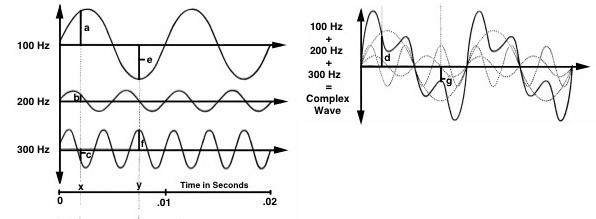
\includegraphics[scale=2]{img/fourier_transform.jpg}

\proposition{Frequency in Images}
\textit{Frequency in Images} is measured as the rate of change in intensity along a given line on the image.\\

\remark{Fourier Transform on Frequency in Images}
If we read the intensity values along a single row or column we can produce a sinusoidal wave which generalises the distribution \& then perform a \textit{Fourier Transform}.\\

\definition{2D Discrete-Space Fourier Transform}
Images can be considered as 2-Dimensional discrete space. Let $f(x,y)$ be the intensity of the pixel at position $(x,y)$. 2D Discrete-Space Fourier Transforms have two variables: $u\in[-\pi,\pi)$ for the vertical frequency; and, $v\in[-\pi,\pi)$ for the horizontal frequency.
\[\begin{array}{rcl}
\underbrace{F(u,v)}_{\text{Fourier Space}}&=&{\displaystyle\sum_{y=0}^{m-1}\sum_{x=0}^{n-1}f(x,y)e^{i(ux+vy)}}\\
&=&{\displaystyle\sum_{y=0}^{m-1}\sum_{x=0}^{n-1}f(x,y)\left[\cos(ux+vy)+\sin(ux+vy)\right]}
\end{array}\]
\nb $F(u,v)$ is a complex number.\\

\proposition{Interpretations of 2D Fourier Transform}
Since $F(u,v)$ is a complex number we cannot plot it exactly. Thus we consider
\begin{enumerate}[label=\roman*)]
	\item $\text{Magnitude},\ |F(u,v)|:=\sqrt{F_\text{r}(u,v)^2+F_\text{i}(u,v)^2}$, and
	\item $\text{Phase Angles},\ \theta(u,v):=\tan^{-1}\left(\dfrac{F_\text{i}(u,v)}{F_\text{r}(u,v)}\right)$
\end{enumerate}

\remark{Expressing $F(u,v)$ in Polar Cordinates}
$$F(u,v)=|F(u,v)|e^{i\theta(u,v)}$$

\remark{Plotting Magnitude, $|F(u,v)|$}
On the left we have a gray scale image \& on the right we have the magnitude of a fourier transform on this image. On the right hand image the $y$-axis is $u\in[-\pi,\pi)$ and the $x$-axis is $v\in[-\pi,\pi)$. We see lots of straight lines since a linear transformation on $F(u,v)=F(au,av)\ \forall\ a\in\mathbb{R}$. Each line can be interpreted as the frequency of intensity for lines in the left hand image which are parallel to it.\\
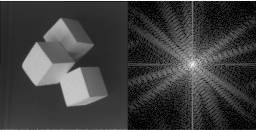
\includegraphics[scale=3]{img/fourier_transform_magnitude.jpg}\\
%TODO interpretting

\theorem{Convolution Theorem}
Let $f$ be an image, $g$ be a kernel, $F$ be the result of a fourier transform on $f$ and $G$ be a kernel. Then
$$h=f*g\Longleftrightarrow H=FG$$

\proof{Convolution Theorem}
\[\begin{array}{rcl}
h(x)&=&f(x)*g(x)\\
&=&\sum_yf(x-y)g(y)\\
H(u)&=&\sum_x\left(\sum_yf(x-y)g(y)\right)e^{iux}\\
&=&\sum_xg(y)\sum_xf(x-y)e^{iux}\\
&=&\sum_yg(y)\left(F(u)e^{iux}\right)\\
&=&\sum_yg(y)e^{iuy}F(u)\\
&=&G(u)\cdot F(u)\\
&=&F(u)\cdot G(u)
\end{array}\]

\definition{Butterworth's Low Pass Filter}
\textit{Butterworth's Low Pass Filter} is a \textit{Signal Processing Filter} designed to have a frequency response which is as flat as possible. It appears to soften an image
$$H(u,v)=\frac{1}{1+\left(\dfrac{r(u,v)}{r_0}\right)^{2n}}\text{ of order $n$}$$

\definition{Butterworth's High Pass Filter}
\textit{Butterworth's High Pass Filter} is a \textit{Signal Processing Filter} designed to have a frequency response which is as flat as possible. It appears to sharpen an image
$$H(u,v)=\frac{1}{1+\left(\dfrac{r_0}{r(u,v)}\right)^{2n}}\text{ of order $n$}$$

\section{Edges \& Shapes}

\subsection{Edge Detection}

\remark{Edges are Useful}
Edges are one of the best features to identify an object with. This \textit{Edge-Detection} is a useful thing to be able to do.

\definition{Edge}
An \textit{Edge} is a sharp change in image brightness. Edges are produced by object boundaries, patterns \& shadows, this can lead to us finding \textit{Nusiance Edges} which do not help achieve our goal.\\

\example{Edge Detection}
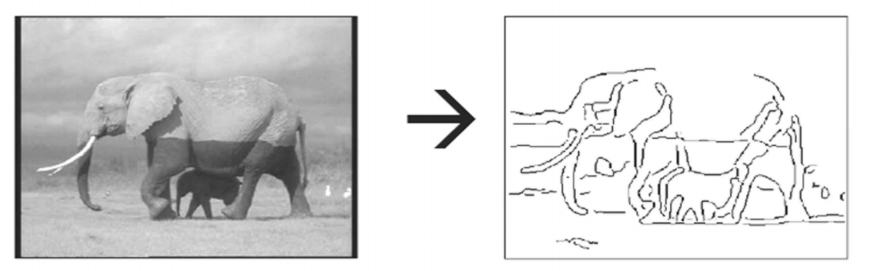
\includegraphics[scale=.7]{img/edgeDetection.png}

\remark{Uses of Edges}
\textit{Edges} are used for
\begin{enumerate}[label=\roman*)]
	\item Segmentation - Finding object boundaries;
	\item Recognition - Extracting patterns;
	\item Motion Analysis - Finding reliable tracking regions.
\end{enumerate}

\remark{Edge Detection Strategy}
In order to find edges we want to determine the \textit{rate of change} in a pixel's neighbourhood

\definition{Image Gradient}
\textit{Image Gradient} is a vector which gives the direction of greatest change in intensity at a specific pixel. For a pixel at $(x,y)$ with $f:\reals\times\reals\to\reals$ mapping to the intensity the \textit{Image Gradient} is
$$\nabla f(x,y):=\begin{pmatrix}
\frac{\partial f}{\partial x}\\
\frac{\partial f}{\partial y}
\end{pmatrix}$$
\nb Generally denoted by $\Psi$.\\

\definition{Angle of Gradient}
$$\Psi:=\tan^{-1}\left(\dfrac{\partial f/\partial y}{\partial f/\partial x}\right)$$

\definition{Edge Direction}
\textit{Edge Direction} for a specific pixel is the direction of an edge, it is perprendicular/orthogonal to the \textit{Image Gradient}.\\
\nb Generally denoted by $\Phi$.\\
$$\Phi:=\Psi-\frac{\pi}{2}=\tan^{-1}\left(\dfrac{\partial f/\partial y}{\partial f/\partial x}\right)-\dfrac{\pi}{2}$$

\definition{Image Gradient Magnitude}
\textit{Magnitude} measures the magnitude of the growth.
$$|\nabla f(x,y)|:=\sqrt{\left(\dfrac{\partial f}{\partial x}\right)^2+\left(\dfrac{\partial f}{\partial y}\right)^2}$$

\proposition{Estimating $\nabla f$}
We can define $\frac{\partial f}{\partial x}$ and $\frac{\partial f}{\partial y}$ to be matrices, rather than typical derivatives, in order to produce estimates for the \textit{Image Gradient} which can be used to analyse an image by convolution. We can then combine the results in order to analyse \textit{Image Gradient Angle} and \textit{Magnitude}. Consider
$$\dfrac{\partial f}{\partial x}=\begin{pmatrix}-1&0&1\\-1&0&1\\-1&0&1\end{pmatrix}\text{ and }\dfrac{\partial f}{\partial y}=\begin{pmatrix}-1&-1&-1\\0&0&0\\1&1&1\end{pmatrix}$$
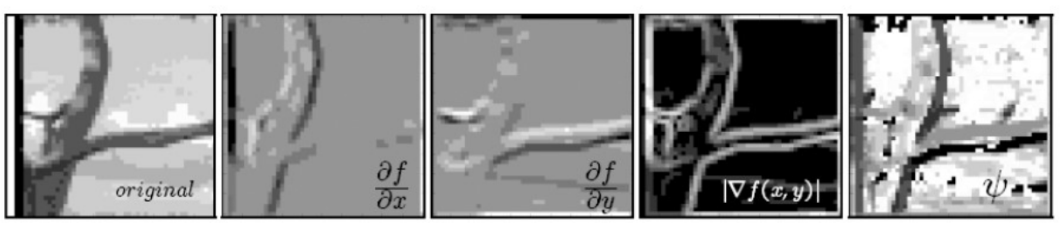
\includegraphics[scale=.5]{img/gradientExtractionByFiltering.png}

\definition{Prewitt Operator}
\textit{Prewitt Operator}s are a set of $3\times3$ kernels used for estimating the \textit{Image Gradient}. There are 8 \textit{Prewitt Operators}, each in a different direction\\
\begin{tabular}{|c|c|c|c|}
\hline
$\begin{pmatrix}
1&1&1\\
0&0&0\\
-1&-1&-1
\end{pmatrix}$&
$\begin{pmatrix}
0&1&1\\
-1&0&1\\
-1&-1&0
\end{pmatrix}$&
$\begin{pmatrix}
-1&0&1\\
-1&0&1\\
-1&0&1
\end{pmatrix}$&
$\begin{pmatrix}
-1&-1&0\\
-1&0&1\\
0&1&1
\end{pmatrix}$\\
\hline
$\begin{pmatrix}
-1&-1&-1\\
0&0&0\\
1&1&1
\end{pmatrix}$&
$\begin{pmatrix}
0&-1&-1\\
1&0&-1\\
1&1&0
\end{pmatrix}$&
$\begin{pmatrix}
1&0&-1\\
1&0&-1\\
1&0&-1
\end{pmatrix}$&
$\begin{pmatrix}
1&1&0\\
1&0&-1\\
0&-1&-1
\end{pmatrix}$\\
\hline
\end{tabular}\\

\remark{Alternative estimates of $\nabla f$}
Instead of weighting all pixels in a given direction equally, we may want to weight central ones more heavily. This is since the central pixels are geometrically closer to the pixel which is being acted upon \& such should better describe it.
$$\dfrac{\partial f}{\partial x}=\begin{pmatrix}
-1&0&1\\
-2&0&2\\
-1&0&1
\end{pmatrix}\quad\dfrac{\partial f}{\partial y}=\begin{pmatrix}
1&2&1\\
0&0&0\\
-1&-2&-1
\end{pmatrix}$$
\nb This is called the \textit{Sobel Filter}.

\subsection{Shapes}

\definition{Hough Transform}
A \textit{Hough Transform} is used to find lines which best explain the set of edge points given to it. \textit{Hough Transform}s are centred around the premise that lines can be described by ${\rho=x\cos\theta+y\sin\theta}$ where either $(x,y)$ is fixed, or $(\rho,\theta)$ is fixed.\\
Suppose we are given an edge point $(x_0,y_0)$, we are now dealing with the case where $(\rho,\theta)$ are variable. Plot all the combinations of $(\rho,\theta)$ than produce lines which pass through $(x_0,y_0)$ produces a sinusoidal wave.\\
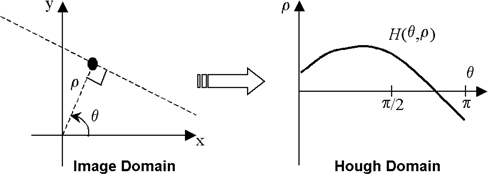
\includegraphics[scale=.7]{img/houghTransform.png}

\proposition{Line Detection Algorithm}
Below is an algorithm which uses the \textit{Hough Transform} on a set of edge points in order to detect lines in an image
\begin{enumerate}[label=\roman*)]
	\item Make available an $n=2$ dimensional array, $H(\rho,\theta)$, to be used for the parameter space;
	\item Find the \textit{Gradient Image}, $G(x,y)$;
	\item For any pixel $(x_0,y_0)$ where $|G(x_0,y_0)|>T_s$ (some threshold value) increment all values of $H(\rho,\theta)$ where $(\rho,\theta)$ satisfy $\rho=x_0\cos\theta_0+y_0\sin\theta_0$.
	$$\forall\ \rho,\theta\text{ where }\rho=x_0\cos\theta_0+y_0\sin\theta_0\text{ do }H(\rho,\theta)+=1$$
	\item Any $(\rho,\theta)$ where $H(\rho,\theta)>=T_h$ (another threshold value) represent a straight line which has been detected in the image.
\end{enumerate}

\propositionn{Circle Detection Algorithm}
\begin{enumerate}[label=\roman*)]
	\item Make available an $n=3$ dimensional array, $H(x,y,r)$, to be used for the parameter space;
	\item Find the \textit{Gradient Image}, $G(x,y)$;
	\item For any pixel $(x_0,y_0)$ where $|G(x_0,y_0)|>T_s$ increment all $H(x,y,r)$ which satisfy
	$$\forall\ r\text{ where }x_0=x+r\cos\Phi\text{ and }y_0+y+r\sin\Phi$$
	\item Any $(x,y,r)$ where $H(x,y,r)>T_h$ represents a circle with radius $r$ and centre $(x_0,y_0)$
\end{enumerate}

\definition{General Hough Transform}
A \textit{Genereal Hough Transform} is used to describe general shapes.
\begin{enumerate}[label=\roman*)]
	\item Find the \textit{Gradient Image}, $G(x,y)$.
	\item Define a set of points $\phi_i:=\frac{pi}{i}$ for $i\in[1,k]$ and create a table using $\phi_1,\dots,\phi_k$ as indexes.
	\item Define a reference point $(x_c,y_c)$ to act as a \textit{centre of mass}.
	\item For any given edge point $(x_0,y_0)$ find
	$$r=\sqrt{(x_0-x_c)^2+(y_0-y_c)^2},\ \beta=\tan^{-1}\left(\dfrac{y_0-y_c}{x_0-x_c}\right)\text{ and }\Phi_{(x_0,y_0)}\text{ in }G(x,y)$$
	\item Round $\Phi_{(x_0,y_0)}$ to the nearest $\phi_i$ and insert $(r,\beta)$ into the table at $\phi_i$
\end{enumerate}

\propositionn{General Shape Detection Algorithm}
\begin{enumerate}[label=\roman*)]
	\item Prepare $2$ dimensional array $H(x_c,y_c)$ for the parameter space (Set of all possible centre of masses).
	\item $\forall\ (x_0,y_0)$ where $|G(x_0,y_0)|>T_s$ find the table entry, $\phi_i$, closest to $\Phi_{(x_0,y_0)}$.
	\item $\forall\ (r_j,\beta_j)$ in the table entry find
	$$x_c=x+r\cos\beta\text{ and }y_c=y+r\sin\beta$$
	Increment $H(x_c,y_c)$.
	\item All $(x_c,y_c)$ where $H(x_c,y_c)>T_h$ represents the locations of centre of masses for occurances of the shap, in the image.
\end{enumerate}

\remark{Issues with \textbf{Proposition 4.4}}
The algorithm defined in \textbf{Proposition 4.4} only detects shapes of the same \textit{scale} and \textit{orientation} as the original image. To counter this we introduce two new variables to the parameter space: $S$, a scaling factor; and, $\theta$, an orientation factor.
\begin{enumerate}[label=\roman*)]
	\item Prepare $4$ dimensional array $H(x_c,y_c,S,\theta)$ for the parameter space (Set of all possible centre of masses, scales \& orientations).
	\item $\forall\ (x_0,y_0)$ where $|G(x_0,y_0)|>T_s$ find the table entry, $\phi_i$, closest to $\Phi_{(x_0,y_0)}$.
	\item $\forall\ (r_j,\beta_j)$ in the table entry find
	$$x_c=x+rS\cos(\beta+\theta)\text{ and }y_c=y+rS\sin(\beta+\theta)$$
	Increment $H(x_c,y_c,S,\theta)$.
	\item All $(x_c,y_c)$ where $H(x_c,y_c,S,\theta)>T_h$ represents the locations of centre of masses, scaling factors \& orientations for occurances of the shape in the image.
\end{enumerate}

\section{Image Segmentation}

\definition{Image Segmentation}
\textit{Image Segmentation} is the process of partitioning the pixels in an image into homogenous regions. This may wrt colour, texture, object.\\

\remark{Usefulness of Image Segmentation}
\textit{Image Segmentation} is useful since it simplifies an image from millions of pixels into a few regions making computation much easier.\\

\definition{Gestalt Rules for Grouping \& Segmentation}
It is useful to consider the different ways in which we can group objects.\\
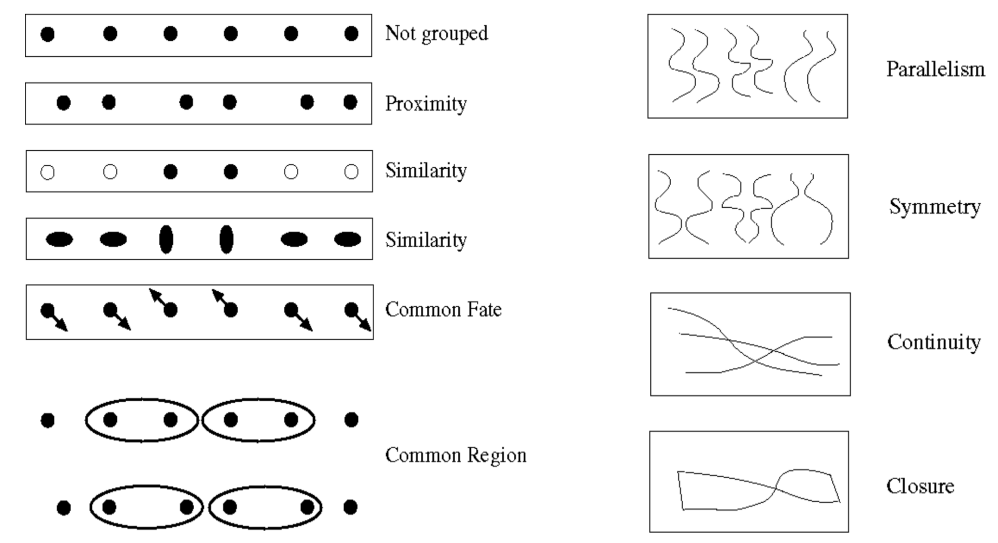
\includegraphics[scale=.5]{img/gestalt.png}

\remark{Perfect Image Segmentation is hard}
It is hard to achieve perfect \textit{Image Segmentation} since pixels may straddle the boundary of objects \& thus not truely belong to any object. Noise, non-uniform illumination, occlusions etc. will also cause problems.\\

\definition{Over-Segmentation}
\textit{Over-Segmentation} is when an image is segmented into too many regions \& loses the efficienies gained by the simplication of \textit{Image Segmentation}.\\

\example{Over-Segmentation}
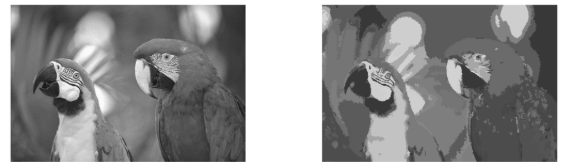
\includegraphics[scale=1]{img/overSegmentation.png}

\definition{Under-Segmentation}
\textit{Uner-Segmentation} is when an image is segmented into too few regions \& too much information is lost.\\

\example{Under-Segmentation}
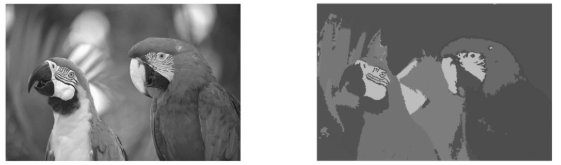
\includegraphics[scale=1]{img/underSegmentation.png}

\proposition{Segmentation Technique Types}
There are several groups of techniques that can be used for \textit{Image Segmentation}
\begin{enumerate}[label=\roman*)]
	\item Thresholding. Categorise pixels wrt intensity.
	\item Edge-Based. Region boundaries are produced using an edge map.
	\item Region-Based. Regions are grown from seed pixels or using split-merge techniques.
	\item Clustering \& Statistical. Global partioning, oftern based around histograms. (\eg K-means).
	\item Topographic (OUT OF SCOPE). Stepwise simplications that take spatially wider image configurations into account.
\end{enumerate}

\proposition{Thresholding Image Segmentation}
\textit{Thresholding} is a good technique when trying to distinguish dark objects(background) from bright objects (foreground). One possible algorithm is
\begin{enumerate}[label=\roman*)]
	\item Choose a threshold value $T$.
	\item For each pixel:
	\begin{enumerate}
		\item If the brighness is less than $T$ map to $0$ (black).
		\item else, map to $255$ (white).
	\end{enumerate}
\end{enumerate}

\remark{Choosing Threshold Value}
Choosing a value for \textit{Thresholding} is important since if it is too high then the background pixels are classified as the foreground. And visa-versa for too low.\\

\proposition{Choosing Threshold Value}
There are several techinques used for choosing \textit{Threshold Value}. By consider the histogram of an image's intensity we can produce regions for classification.
\begin{enumerate}[label=\roman*)]
	\item Make an initial estimate for threshold $T$.
	\item Segment the image using $T$: Let $G_1$ be the pixels with intensity $>T$; and $G_2$ be the pixels with intensity $<T$.
	\item COmpute the average intensity values $m_1$ \& $m_2$ for $G_1$ \& $G_2$ respectively.
	\item Compute a new threshold value $T=\frac{1}{2}(m_1+m_2)$.
	\item Repeat \textbf{ii)-iv)} until convergence.
\end{enumerate}

\proposition{Edge-Based Segmentation}
When performing \textit{Edge-Based Image Segmentation} we want to detect strong edges that are relevant to the objet we wish to detect. There are several techniques for assessing the strength of an edge, but generally we wish to remove edges that are isolated of irrelevant to an object. One valid technique is edge relaxation where we change the strength of an edge depending upon its 6 neighbour edges.\\
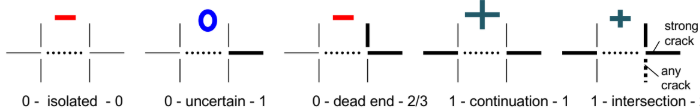
\includegraphics[scale=.7]{img/edgeRelaxation.png}.\\

\proposition{Region Growing-Seed Pixel}
A function is required to analyse the homogeneity of two pixels $(s,p)\to\{0,1\}$.
\begin{enumerate}[label=\roman*)]
	\item Choose an initial seed pixel;
	\item Consider the neighbouring pixels:
	\begin{enumerate}
		\item If it is close to seed pixel, add to region \& to queue to be analysed.
		\item Else, do nothing with it.
	\end{enumerate}
	\item Repeat \textbf{ii)} until there are no pixels left in the queue to be analysed.
\end{enumerate}
\nb You may wish to add a final step to remove small regions.\\

\proposition{Split \& Merge Segmentation}
Let $H$ be a function to analyse the homogeneity of a region $(R)\to\{0,1\}$
\begin{enumerate}[label=\roman*)]
	\item Let $R_0$ represent the entire image.
	\item If $H(R_i)=0$ (\ie is inhomogenous) then split it into four regions.
	\item Repeat \textbf{ii)} until all regions are homogenous.
	\item Merge all subregions that satisfy $H(R_i\cup R_j)=1$ (\ie are homogeneous)
\end{enumerate}

\proposition{Clustering Segmentation}
If we map the RGB values of an image into the 3D real space we can we clustering algorithms to produce $k$ clusters. We then map back to the pixel space using each cluster as a segment.\\
\nb Look at k-means clustering.

\section{Classical Object Detection}

\remark{Classical Object Detection}
In this course we only conver \textit{Classical Object Detection}. This technique came to prominence with the 2001 paper \textit{First Real-Time Detection Method: Viola \& Jones' - 2001} and was the industry standard for 10+ years. Now there are methods which use deep learning techniques.\\

\definition{Object Detection}
\textit{Object Detection} bridges the semantic gap between [ixel values \& meaningful objects by grouping pixels and classifying. This is a difficult problem.\\

\remark{Failings of Shape Detection for Object Detection}
Typically using classical \textit{Shape Detection} \& \textit{Segmentation} does not work for real world applications of \textit{Object Detection} due
\begin{enumerate}[label=\roman*)]
	\item High Intra-Class \& Low Inter-Class variance;
	\item Classes are rarely well defined;
	\item Variations in illumination, scale, pose, deformation, occlusion etc.
\end{enumerate}

\remark{Shift-Scale Invariance}
We require \textit{Object Detection} algorithms to be shift \& scale invariant so it can detect objects of any size at any point in the image.\\

\definition{Sliding Window Detectors}
\textit{Sliding Window Detectors} ensure shift \& scale invariance by setting a minimum size to check (say $20\times20$px) and shifts the region it checks by 1px right-to-left, top-to-bottom until the whole is checked. They then increase the size of the region it checks (say $10\%$) and repeats the shifting. It does this until the size of the region it checks exceeds the size of the image.\\
\nb This technique does not work in real-time due to its high computation complexity.\\

\definition{Haar-Like Features}
\textit{Haar-Like Features} are features of digital images used in \textit{Object Detection}. They define a set of adjacent rectangles and assigns them to either be \textit{light} or \textit{dark} regions. It then returns a value, the average gray value of the light region less the average gray value of the dark region. This value is then compared to a threshold value to determine whether the feature occurs in the image.\\

\proposition{Haar-Like Feature Types}
There are a finite set of \textit{Haar-Like Features Types}\\
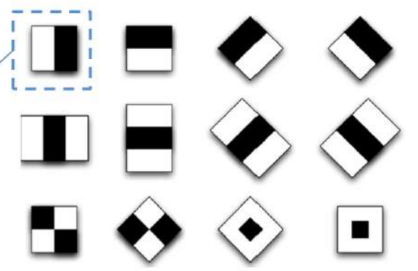
\includegraphics[scale=.6]{img/haar.png}\\

\definition{Image Integral}
The \textit{Integral} of an image $I$ is the image $J$ where $J(x,y)=\sum_{i=0}^x\sum_{j=0}^yI(i,j)$. \ie Each pixel value is the sum of all pixels between it an the origin, inclusive.\\

\proposition{Calculating Image Integral}
Let $I$ be an image then we can calculate the \textit{Integral} of $J$ in \textit{Linear Time} using the following formulae
\[\begin{array}{l}
A(x,-1)=0\\
A(x,y)=A(x,y-1)+I(x,y)\\
J(-1,y)=0\\
J(x,y)=J(x-1,y)+A(x,y)
\end{array}\]

\theorem{Integration Rule of Convolution}

\proposition{Calculating the Average Pixel Value of a Large Block}
Calculating the average pixel value of a large block can be very slow if the region is very large. Here is a technique that can do it by only quering 4 values.
\begin{enumerate}[label=\roman*)]
	\item Create a matrix which is the same size as the image.
	\item Encode the matrix st its values are 1 in the region we want to check \& 0 everywhere else.
	\item Double Differentiate this matrix to produce $I''$
	\begin{enumerate}
		\item First, horizontally by applying $\begin{pmatrix}0&-1&1\end{pmatrix}$ to every pixel.
		\item Then, vertically by applying $\begin{pmatrix}0\\-1\\1\end{pmatrix}$ to every pixel.
	\end{enumerate}
	This leaves us with four non-zeros values (two $1$s and two $-1$s).7
	\item Calculate the image integral $J$.
	\item Return $\sum_i\sum_j I''(i,j)\times J(i,j)$\\
	\nb This can be simplied to just be the four non-zero terms in $I''$.
\end{enumerate}

\proposition{Training Data}
Two categories of \textit{Trainging Data} should be provided: \textit{Positive Samples}, images of the object you wish to classify' and, \textit{Negative Samples}, images which do not contain the object. These should be labled $(x_i,y_i)$ with $y_i=0,1$ for \textit{Negative} and\textit{Positive Samples} respectively.\\

\definition{Adaboost}
\textit{Adaboost} (Short for \textit{Adaptive Boosting}) is a machine learning algorithm.\\
Let $(x_1,y_1),\dots,(x_n,y_n)$ with $y_i=0,1$ for negative \& positive samples respectively
\begin{enumerate}[label=\roman*)]
	\item Initalise weights $w_{1,i}=\begin{cases}\frac{1}{2^m},&\text{if }y_i=0\\\frac{1}{2^l},&\text{if }y_i=1\end{cases}$ where $m$ is the number of negative samples \& $l$ is the number of positive samples.
	\item For $t=1,\dots,T$ where $T$ is the number of features you wish to find
	\begin{enumerate}
		\item Normalise the weights st $w_t$ is a probability distribution
		$$w_{t,i}:=\frac{w_{t,i}}{\sum_{j=1}^nw_{t,j}}$$
		\item For each feature, $j$, train a classifier $h_j$ which is restricted to using a single feature (Haar-Like Feature). Calculate the error wrt $w_t$
		$$e_j=\sum_iw_i|h_j(x_i)-y_i|$$
		\item Choose the classifier, $h_t$, with the lowest error $e_t$.
		\item Update the weights
		$$w_{t+1,i}=w_{t,i}\left(\frac{e_t}{1-e_t}\right)^{1-e_i}$$
		where $e_i=0$ if sample $x_i$ is classified correctly and $e_i=1$ otherwise
	\end{enumerate}
	\item The final strong classifier is
	$$h(x)=\begin{cases}1&\sum_{i=1}^T\log\left(\frac{e_t}{1-e_t}\right)h_t(x)\geq\frac{1}{2}\sum_{t=1}^T\log\left(\frac{1-e_t}{e_t}\right)\\0&\text{otherwise}\end{cases}$$
\end{enumerate}

\section{Motion}

\definition{Video Sequences}
A video can be considered as a series of matrices, each representing an image at a different point in time. The time difference between consecutive matrices will be constant, $\Delta t$ seconds.\\
Define $I(x,y,t)$ to be the intensity of the pixel at position $(x,y)$ at time $t$.\\

\definition{Frame Rate}
\textit{Frame Rate} is the number of images per second in a video. Typically measured in FPS (\textit{Frames Per Second}), this is equivalent to Hz.
$$\text{Frame Rate}=\frac{1}{\Delta T}$$
\nb Typical frame rates are $24fps,\ 30fps\ \&\ 60fps$.\\

\definition{2D Tracking}
\textit{2D Tracking} is tracking how an object moves in a two dimensional plane. The object may really be moving a three dimensionial plane, but we only care about its movement in a specified 2D plane.\\
This means the object has 3 attributes: x position, y position \& orientation. Scale can be considered too.\\

\example{2D Tracking}
In the below image the path the pen has taken in the plane parallel to the camera has been tracked. The pen is actually moving in 3-dimensions, but we are ignoring depth in this example.\\
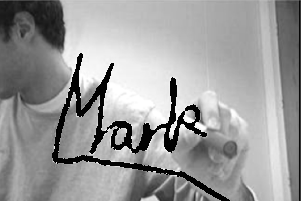
\includegraphics[scale=1]{img/2dtracking.png}

\definition{3D Tracking}
\textit{3D Tracking} is used to track an object's movement in a three dimensional space. This means an object has six factors: x,y,z positions and rotation in the x,y,z directions. Scale can be considered too.

\example{3D Tracking}
In the below image a printer is tracker so that a skeleton of it can be mapped to it.\\
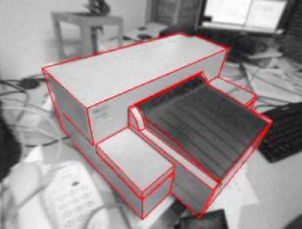
\includegraphics[scale=1]{img/3dtracking.png}

\definition{Simultaneous Localisation and Mapping}
\textit{Simultaneous Localisation and Mapping}, SLAM, is the process of constructing and updating a map of an unknown enviroment while tracking the camera's position within it.\\
\nb This can be made easier by using a depth sensor.\\

\definition{Perspective Projection Equations}
Suppose a 3D point $\textbf{P}=(X,Y,Z)$, which sits on the surface of an object, is projected to a point in two dimensions, $\textbf{p}=(x,y,f)$ ($f$ is the distance of the 2D plane from the camera). Then, by similar triangles
$$x=\frac{fX}{Z}\text{ and }y=\frac{fY}{Z}$$
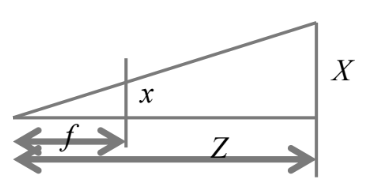
\includegraphics[scale=.5]{img/perspectiveprojectionequations.png}

\definition{Rotation Matrices}
A \textit{Rotation Matrix} can be applied to a position, by matrix-multiplication, to perform a rotation on that position. A \textit{Rotation Matrix}, $R$ can be broken down into \textit{Rotation Matrices} which represent the rotation about each axis. In three-dimensions this means $R=R_XR_YR_Z$.\\
\nb \textit{Rotation Matrices} are $n\times n$ in $n$-dimensional space.\\

\remarkk{3D Rotation Matrices}
$$R_X(\theta)=\begin{pmatrix}1&0&0\\0&\cos\theta&-\sin\theta\\0&\sin\theta&\cos\theta\end{pmatrix}\quad R_Y(\theta)=\begin{pmatrix}\cos\theta&0&\sin\theta\\0&1&0\\-\sin\theta&0&\cos\theta\end{pmatrix}\quad R_Z(\theta)=\begin{pmatrix}\cos\theta&-\sin\theta&0\\\sin\theta&\cos\theta&0\\0&0&1\end{pmatrix}$$

\proposition{Rotation Matrices for small $\theta$}
When $\theta$ is small we can approximate $\sin\theta\approx\theta$ and $\cos\theta\approx1$. Thus
$$R_X(\theta)=\begin{pmatrix}1&0&0\\0&1&-\theta\\0&\theta&1\end{pmatrix}\quad R_Y(\theta)=\begin{pmatrix}1&0&\theta\\0&1&0\\-\theta&0&1\end{pmatrix}\quad R_Z(\theta)=\begin{pmatrix}1&-\theta&0\\\theta&1&0\\0&0&1\end{pmatrix}$$

\definition{Rigid Object}
A \textit{Rigid Object} is one which does not change in shape, only scale \& rotation.\\

\proposition{3D Rigid Motion}
Consider a \textit{Rigid Object} \& a point on that object $\textbf{P}$.\\
If the object is moved st point $\textbf{P}$ is now at position $\textbf{P}'$ then we can describe $\textbf{P}'$ in terms of $\textbf{P}$ by defining a translation matrix $T$ and a rotation matrix $R$.
$$\textbf{P}'=R\textbf{P}+T$$
\nb $\textbf{P},\ \textbf{P}'\ \&\ T$ are $3\times1$ matrices and $R$ is a $3\times3$ matrix.\\

\proposition{3D Motion Field}
Consider a \textit{Rigid Object} \& a point on that object $\textbf{P}$.\\
Let $V$ be the vector which represents the translation from $\textbf{P}$ to $\textbf{P}'$. We have
$$V=\lim_{\Delta t\to0}[\textbf{P}'-\textbf{P}]=\lim_{\Delta t\to0}[(R-I)\textbf{P}+T]$$
We note that for small $\theta_X,\theta_Y\ \&\ \theta_Z$
$$R=\begin{pmatrix}1&-\theta_Z&\theta_Y\\\theta_Z&1&-\theta_X\\-\theta_Y&\theta_X&1\end{pmatrix}$$
Thus
\[\begin{array}{rcccl}
\frac{dX}{dt}&=&V_X&=&\theta_YZ-\theta_ZY+T_X\\
\frac{dY}{dt}&=&V_Y&=&\theta_ZX-\theta_XZ+T_Z\\
\frac{dZ}{dt}&=&V_Z&=&\theta_XY-\theta_YX+T_Z
\end{array}\]
\nb Here $(\theta_X,\theta_Y,\theta_X)$ is called the \textit{Angular Velocity} and $(T_X,T_Y,T_Z)$ is called the \textit{Rectilinear Velocity} since we are taking the limit as $\Delta t$ tends to 0.\\

\proposition{2D Motion Field Equations}
Consider a point $\textbf{p}=(x,y,f)$ which represents a 2D projection of a point $\textbf{P}=(X,Y,Z)$.\\
Then
\[\begin{array}{rcl}
v_x&=&\frac{d}{dt}x\\
&=&\frac{d}{dt}\left(\frac{fX}{Z}\right)\\
&=&f\frac{V_XZ-XV_Z}{Z^2}\text{ by quotient rule}
\end{array}\]
Substituting $V_X,V_Y,V_Z$ for the definitions in \textbf{Proposition 7.3} we get
$$v_x=\frac{fT_X-xT_Z}{Z}+f\theta_Y-\theta_Zy-\frac{\theta_Xxy-\theta_Yx^2}{f}\text{ and }v_y=\frac{fT_Y-yT_Z}{Z}-f\theta_X+\theta_Zx+\frac{\theta_Yxy-\theta_Xy^2}{f}$$
We can recognise two components of these equations: Translation, terms involving $T$; and Rotation, terms involving $\theta$.
\newpage
\setcounter{section}{-1}

\section{Reference}

\subsection{Definitions}

\definition{Connectivity}
When analysing a pixel there are several ways to consider its adjacent neighbourhood.
\begin{itemize}
	\item[-] 4-Connectivity. The pixels above, below, left \& right.
	\item[-] 8-Connectivity. Above, below, left, right \& single step diagonals.
\end{itemize}

\definition{Kernel}
A \textit{Kernel} is a small matrix used in convolution. Typically $3\times3$ or $5\times5$. \textit{Kernels} can be defined for blurring, sharpening, embossing, edge detection \& more
\nb This definition only applies to image processing \& is different from the definition in linear algebra.

\end{document}